%узнать о изменении головы в документах / вставить ссылки на изображение / доделать / ...

\documentclass[12pt, letterpaper]{article}
\usepackage[utf8]{inputenc}

%Graphicx 
\usepackage{graphicx}
\usepackage{float}

% Header & Footer 
\usepackage{fancyhdr}
\pagestyle{fancy}

%First/Info page
\begin{document}
\begin{titlepage}
	\begin{center}	
	\line(1,0){300} \\
	[0.25in]
	\huge{\bfseries \huge Spring boot ako ľahký nastroj pre vašu stránku} \\
	[2mm]
	\line(1,0){200} \\
	[2cm]
	\textsc{\large Slovenská technická univerzita v Bratislave \\ Fakulta informatiky a informačných technológií} \\
	[8cm]
	\end{center}
	\begin{flushright}
	\textsc{\large Andrei Trusau \\ xtrusau@stuba.sk\\ ID: 116317 \\ 02.11.2021 \\}
	\end{flushright}
	\newpage
\end{titlepage}

% Spring logo
\begin{figure}[H]
	\centering
	
\includegraphics[height=1in]{Spring_logo.png}
	\caption[Optional caption]{spring} %add link
\end{figure}

%This is table of content
\tableofcontents
\thispagestyle{empty}
\cleardoublepage
\setcounter{page}{1}

%First abstract (Page 1)
\section{Abstrakt}\label{sec:intro}
Spring je veľmi populárne vývojové prostredie založené na jazyku Java, ktoré sa používa na vytváranie webových a podnikových aplikácií. Na rozdiel od mnohých iných platforiem, ktoré sa zameriavajú iba na jednu oblasť, Spring poskytuje širokú škálu funkcií, ktoré spĺňajú potreby dnešného podnikania prostredníctvom svojich portfóliových projektov.

Spring framework poskytuje flexibilitu na prispôsobenie bean-komponentov rôznymi spôsobmi, ako je XML, anotácie a JavaConfig. S rastúcim počtom funkcií sa zvyšuje zložitosť a konfigurácia aplikácií Spring sa stáva únavnou a náchylnou na chyby.

Tím Spring vytvoril Spring Boot na riešenie zložitosti konfigurácie. 

Ale predtým, než sa ponoríme do Spring Boot, rýchlo sa pozrieme na Spring, aby sme zistili, aké problémy sa Spring Boot snaží vyriešiť.\\
\newpage

%Second abstract (Page 2)
\section{Ponorime sa do témy Spring}	
Ťažkopádna konfigurácia závislostí spôsobila, že konfigurácia Spring pre podnikové aplikácie je únavná a náchylná na chyby. Platí to najmä pre aplikácie, ktoré využívajú aj viaceré knižnice tretích strán.	

	Ak ste vývojár v jazyku Java, väčšina z vás už o Spring počula a možno ste ju dokonca použili vo svojich projektoch. Spring Boot je jedným z mnohých projektov v ekosystéme Spring, no na rozdiel od väčšiny svojich bratov nerieši žiadny konkrétny problém, skôr predstavuje novú etapu vo vývoji Springu ako celku.
	% 2.1 Abstract and item menu
	\subsection{Konfigurácia Spring}
	Zakaždým, keď vytvoríte ďalšiu podnikovú aplikáciu Java založenú na Spring, musíte na jej konfiguráciu zopakovať rovnaké rutinné kroky:
	
	\begin{itemize}
		\item V závislosti od typu aplikácie, ktorú vytvárate (Spring MVC, Spring JDBC, Spring ORM atď.),musite importovať požadované moduly Spring.
		\item Import knižnice webových kontajnerov (v prípade webových aplikácií)
		\item Importovaťpožadované knižnice tretích strán (napr. Hibernate, Jackson), pričom by ste mali hľadať verzie, ktoré sú kompatibilné so špecifikovanou verziou Spring.
		\item Nakonfiguroť komponenty DAO, ako sú zdroje údajov, správa transakcií atď.
		\item Nakonfiguroť komponenty webovej vrstvy, ako sú: správca zdrojov, prekladač pohľadov.
		\item Definovat triedu, ktorá načíta všetky požadované konfigurácie.
	\end{itemize}
	
	Autori Springu sa rozhodli poskytnúť vývojárom niekoľko utilít, ktoré automatizujú procedúru konfigurácie a urýchľujú proces vytvárania a nasadzovania Spring aplikácií, pod všeobecným názvom Spring Boot. Spring Boot je užitočný projekt, ktorého cieľom je uľahčiť vytváranie aplikácií založených na Spring. Umožňuje vám vytvoriť webovú aplikáciu najjednoduchším spôsobom, čo vyžaduje, aby vývojári vynaložili minimálne úsilie na jej konfiguráciu a písanie kódu.
\newpage

%Third Anstract (Page 3)
\section{Akú úlohu hrá Spring Boot pri tvorbe webových stránok?}
Nie je možné napísať plnohodnotný projekt iba pomocou HTML, CSS a JavaScriptu. Povedzme, že máte jednoduchú prihlasovaciu stránku, kde budete musieť zadať a zobraziť údaje používateľa. Súhlasíte, je veľký problém s nimi pracovať len cez HTML a JavaScript, na to je tu Spring Boot, ktorý predpisuje celú backendovú časť (funkčnosť) projektu.

	Spring Boot je v prvom rade jeden z najrýchlejších spôsobov vytvárania webových aplikácií bez obzvlášť zložitých problémov s načítaním a zápisom konfigurácie servera pre vašu webovú aplikáciu.
	S jeho výberom nastavení možno nebudete vždy súhlasiť, no poskytne vám aspoň funkčný modul. Toto je veľmi užitočný prístup, najmä pre začínajúcich vývojárov, ktorí môžu začať s predvolenými nastaveniami a potom vykonávať zmeny v konfigurácii, keď skúmajú existujúce alternatívy.

% Info about Spring logo
\begin{figure}[H]
	\centering
	\includegraphics[height=2in]{Spring_info.png}
	\caption[Optional caption]{spring\cite{Image_Info}}
\end{figure}

	%3.1 Abstract
	\subsection{Budovanie aplikačnej infraštruktúry}
		Vo väčšine prípadov zmeny predvolených nastavení stačí upraviť súbor POM. Aplikačná infraštruktúra pozostáva z pridávania potrebných modulov do súboru pom.xml:
	
	% POM image 
	\begin{figure}[H]
		\centering
		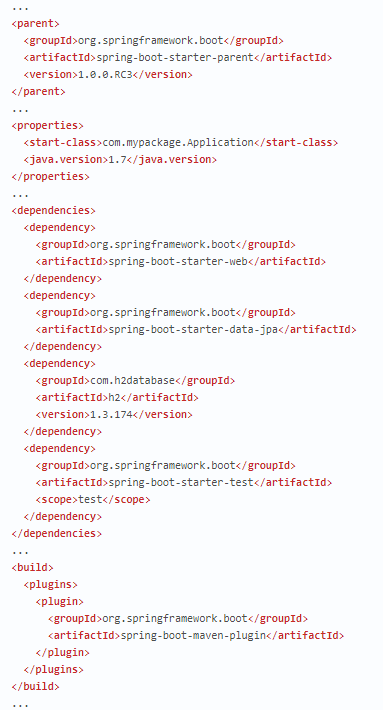
\includegraphics{POM_example.png}
	\end{figure}

.\\
.\\
.\\
.\\
.\\
.\\
to be continued\\
.\\
.\\
.\\
.\\
.\\
.\\

\cleardoublepage
\bibliographystyle{IEEEtran}
\bibliography{zdroje.bib}








\end{document}